\documentclass[journal,12pt,twocolumn]{IEEEtran}

\usepackage{setspace}
\usepackage{gensymb}

\singlespacing


\usepackage[cmex10]{amsmath}

\usepackage{amsthm}

\usepackage{mathrsfs}
\usepackage{txfonts}
\usepackage{stfloats}
\usepackage{bm}
\usepackage{cite}
\usepackage{cases}
\usepackage{subfig}

\usepackage{longtable}
\usepackage{multirow}

\usepackage{enumitem}
\usepackage{mathtools}
\usepackage{steinmetz}
\usepackage{tikz}
\usepackage{circuitikz}
\usepackage{verbatim}
\usepackage{tfrupee}
\usepackage[breaklinks=true]{hyperref}
\usepackage{graphicx}
\usepackage{tkz-euclide}

\usetikzlibrary{calc,math}
\usepackage{listings}
    \usepackage{color}                                            %%
    \usepackage{array}                                            %%
    \usepackage{longtable}                                        %%
    \usepackage{calc}                                             %%
    \usepackage{multirow}                                         %%
    \usepackage{hhline}                                           %%
    \usepackage{ifthen}                                           %%
    \usepackage{lscape}     
\usepackage{multicol}
\usepackage{chngcntr}

\DeclareMathOperator*{\Res}{Res}

\renewcommand\thesection{\arabic{section}}
\renewcommand\thesubsection{\thesection.\arabic{subsection}}
\renewcommand\thesubsubsection{\thesubsection.\arabic{subsubsection}}

\renewcommand\thesectiondis{\arabic{section}}
\renewcommand\thesubsectiondis{\thesectiondis.\arabic{subsection}}
\renewcommand\thesubsubsectiondis{\thesubsectiondis.\arabic{subsubsection}}


\hyphenation{op-tical net-works semi-conduc-tor}
\def\inputGnumericTable{}                                 %%

\lstset{
%language=C,
frame=single, 
breaklines=true,
columns=fullflexible
}
\begin{document}


\newtheorem{theorem}{Theorem}[section]
\newtheorem{problem}{Problem}
\newtheorem{proposition}{Proposition}[section]
\newtheorem{lemma}{Lemma}[section]
\newtheorem{corollary}[theorem]{Corollary}
\newtheorem{example}{Example}[section]
\newtheorem{definition}[problem]{Definition}

\newcommand{\BEQA}{\begin{eqnarray}}
\newcommand{\EEQA}{\end{eqnarray}}
\newcommand{\define}{\stackrel{\triangle}{=}}
\bibliographystyle{IEEEtran}
\providecommand{\mbf}{\mathbf}
\providecommand{\pr}[1]{\ensuremath{\Pr\left(#1\right)}}
\providecommand{\qfunc}[1]{\ensuremath{Q\left(#1\right)}}
\providecommand{\sbrak}[1]{\ensuremath{{}\left[#1\right]}}
\providecommand{\lsbrak}[1]{\ensuremath{{}\left[#1\right.}}
\providecommand{\rsbrak}[1]{\ensuremath{{}\left.#1\right]}}
\providecommand{\brak}[1]{\ensuremath{\left(#1\right)}}
\providecommand{\lbrak}[1]{\ensuremath{\left(#1\right.}}
\providecommand{\rbrak}[1]{\ensuremath{\left.#1\right)}}
\providecommand{\cbrak}[1]{\ensuremath{\left\{#1\right\}}}
\providecommand{\lcbrak}[1]{\ensuremath{\left\{#1\right.}}
\providecommand{\rcbrak}[1]{\ensuremath{\left.#1\right\}}}
\theoremstyle{remark}
\newtheorem{rem}{Remark}
\newcommand{\sgn}{\mathop{\mathrm{sgn}}}
\providecommand{\abs}[1]{\vert#1\vert}
\providecommand{\res}[1]{\Res\displaylimits_{#1}} 
\providecommand{\norm}[1]{\Vert#1\rVert}
%\providecommand{\norm}[1]{\lVert#1\rVert}
\providecommand{\mtx}[1]{\mathbf{#1}}
\providecommand{\mean}[1]{E[ #1 ]}
\providecommand{\fourier}{\overset{\mathcal{F}}{ \rightleftharpoons}}
%\providecommand{\hilbert}{\overset{\mathcal{H}}{ \rightleftharpoons}}
\providecommand{\system}{\overset{\mathcal{H}}{ \longleftrightarrow}}
	%\newcommand{\solution}[2]{\textbf{Solution:}{#1}}
\newcommand{\solution}{\noindent \textbf{Solution: }}
\newcommand{\cosec}{\,\text{cosec}\,}
\providecommand{\dec}[2]{\ensuremath{\overset{#1}{\underset{#2}{\gtrless}}}}
\newcommand{\myvec}[1]{\ensuremath{\begin{pmatrix}#1\end{pmatrix}}}
\newcommand{\mydet}[1]{\ensuremath{\begin{vmatrix}#1\end{vmatrix}}}
\numberwithin{equation}{subsection}
\makeatletter
\@addtoreset{figure}{problem}
\makeatother
\let\StandardTheFigure\thefigure
\let\vec\mathbf
\renewcommand{\thefigure}{\theproblem}
\def\putbox#1#2#3{\makebox[0in][l]{\makebox[#1][l]{}\raisebox{\baselineskip}[0in][0in]{\raisebox{#2}[0in][0in]{#3}}}}
     \def\rightbox#1{\makebox[0in][r]{#1}}
     \def\centbox#1{\makebox[0in]{#1}}
     \def\topbox#1{\raisebox{-\baselineskip}[0in][0in]{#1}}
     \def\midbox#1{\raisebox{-0.5\baselineskip}[0in][0in]{#1}}
\vspace{3cm}
\title{Assignment-4}
\author{Satya Sangram Mishra}
\maketitle
\newpage
\bigskip
\renewcommand{\thefigure}{\theenumi}
\renewcommand{\thetable}{\theenumi}
Download all python codes from 
\begin{lstlisting}
https://github.com/satyasm45/Summer-Internship/tree/main/Assignment-4/Codes
\end{lstlisting}
%
and latex-tikz codes from 
%
\begin{lstlisting}
https://github.com/satyasm45/Summer-Internship/tree/main/Assignment-4
\end{lstlisting}
%
\section{Question No. 2.30}
Find the equation of the parabola with focus $\myvec{2\\0}$ and directrix $\myvec{1&0}\vec{x}=-2$.
%
\section{Explanation}
\begin{definition}
\label{def}
A parabola is a curve where any point is at an equal distance from: a fixed point (the focus $\vec{F}$ ), and. a fixed straight line (the directrix $\vec{n}^T\vec{x}=c$).
\end{definition}
\begin{lemma}
\label{lemma}
The distance of a point $\vec{P}$ from a line $\vec{n}^T\vec{x}=c$ is given by:
\begin{align}
\frac{\abs{c-\vec{P}^T\vec{n}}}{\norm{\vec{n}}}   
\end{align}
\end{lemma}

Using Definition \ref{def} and Lemma \ref{lemma} for any point $\vec{x}$ on parabola we have:
\begin{align}
\norm{\vec{x}-\vec{F}}^2=\frac{({c-\vec{x}^T\vec{n}})^2}{\norm{\vec{n}}^2}\label{eq:1} 
\end{align}

\numberwithin{figure}{section}
\begin{figure}[!ht]
\centering
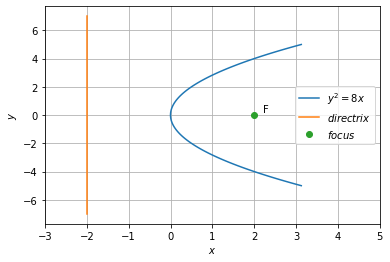
\includegraphics[width=\columnwidth]{figure4}
\caption{Parabola $y^2=8x$ }
\label{fig:parabola}	
\end{figure}


\begin{theorem}
The equation of a parabola with focus $\vec{F}$ ,directrix $\vec{n}^T\vec{x}=c$ and $\lambda=\norm{\vec{n}}^2$ is given by:
\begin{align}
\vec{x}^T(\lambda\vec{I}-\vec{n}\vec{n}^T)\vec{x}+2(c\vec{n}-\lambda\vec{F})^T\vec{x}+\lambda\norm{\vec{F}}^2-c^2&=0
\end{align}
\end{theorem}

\begin{proof}
Using \eqref{eq:1}
\begin{align}
\lambda(\vec{x}-\vec{F})^T(\vec{x}-\vec{F})=(c-\vec{x}^T\vec{n})^2
\\
\lambda(\vec{x}^T\vec{x}-2\vec{F}^T\vec{x}+\norm{\vec{F}}^2)=c^2+(\vec{x}^T\vec{n})^2-2c\vec{x}^T\vec{n}\\
\lambda\vec{x}^T\vec{x}-(\vec{x}^T\vec{n})^2-2\lambda\vec{F}^T\vec{x}+2c\vec{n}^T\vec{x}=c^2-\lambda\norm{\vec{F}}^2\\
\lambda\vec{x}^T\vec{I}\vec{x}-\vec{x}^T\vec{n}\vec{n}^T\vec{x}+2(c\vec{n}-\lambda\vec{F})^T\vec{x}=c^2-\lambda\norm{\vec{F}}^2\\
\vec{x}^T(\lambda\vec{I}-\vec{n}\vec{n}^T)\vec{x}+2(c\vec{n}-\lambda\vec{F})^T\vec{x}+\lambda\norm{\vec{F}}^2-c^2&=0\label{eq:8}
\end{align}
\end{proof}
Given information:
\begin{align}
\vec{F}=\myvec{2\\0},
\vec{n}=\myvec{1\\0},
c=-2\label{eq:9},
\lambda=1
\end{align}


Substituting values of $\vec{F},\vec{n}$,c,$\lambda$ from\eqref{eq:9}:
\begin{align}
\vec{x}^T\myvec{0&0\\0&1}\vec{x}+2\myvec{-4&0}\vec{x}+0&=0\label{eq:11}
\end{align}

Replacing $\vec{x}$ by $\myvec{x\\y}$ in \eqref{eq:11} gives:
\begin{align}
y^2=8x
\end{align}


\end{document}